\chapter{Strongly Anisotropic Systems}
\label{ch5-anis}

By now it should be clear that the notion of scale invariance is a central
tenet of the modern narrative of critical phenomena. This principle show its
true power in the context of conformal invariance. Several critical systems
however are explicitly not scale invariant in its strictest sense. These are
systems out of equilibrium and Theses systems are called strongly anisotropic
systems.

Strongly anisotropic systems are characterized by an \textit{anisotropy
exponent} $\theta$ defined by the relation
\begin{equation}
    C(x, y) = b^{-2x}C(bx, b^\theta y).
\end{equation}
In the case $\theta=1$, isotropy is recovered.

It has been determined that if $\theta = 2/N$, where $N$ is a positive integer,
the systems if invariant under local scale invariance [???], which is the same
principle that motivated the introduction of conformal invariance (which is in
fact the case $N=2$). This observation have been used to successfully study
some anisotropic systems, like the Liftshitz point in the ANNNI [???] and
spherical models [???].


\section{Directed Percolation}
\label{sec:dp}

The percolation model, as described in Section XX, is arguably one of the most
important models for second-order phase transitions, second only to the regal
Ising model. Not surprisingly, several variations of this model have been
proposed in order to explore other other facets of phase transition, like CSA
[???], explosive percolation [???] and invasive percolation [???].

Here we shall describe a variation of the percolation model that is of
particular interest to the study of strongly anisotropic systems. One variant
that is particularly important to the study of anisotropic phase transition is
called \textit{Directed percolation}. It can be seen as a spreading process,
where the flow 

Most recently, experiments and simulations on fluid dynamics indicate
that the transition from laminar to turbulent flow belongs to the
universality class of directed percolation [???].

Owczarek et al.\ found that the hull of a directed percolation cluster
scale as


\begin{figure}
\begin{center}
    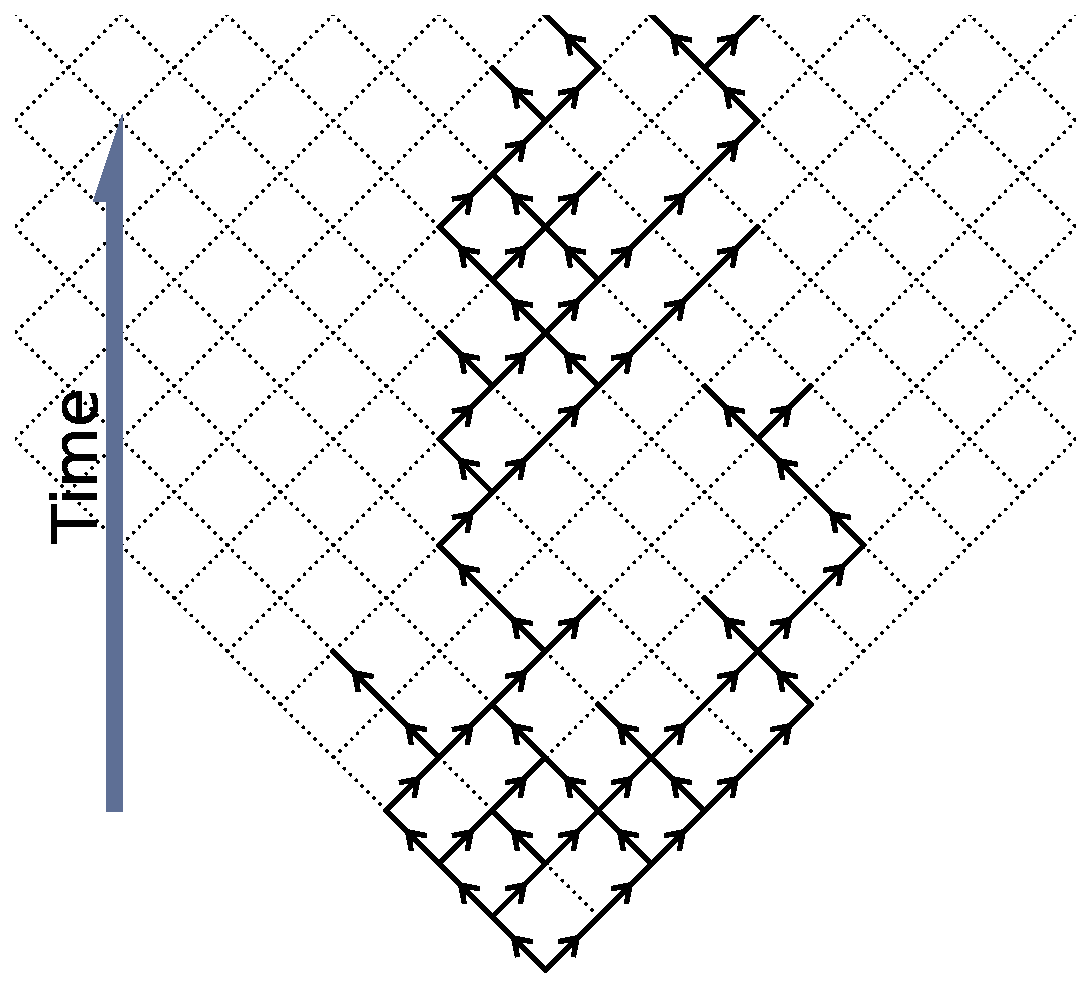
\includegraphics[scale=0.5]{chapters/ch5-anis/figs/dperco_scheme}
\end{center}
\caption{Simple representation of bond directed percolation in a square
    lattice. Here, the time flows upwards (although the time direction can be
    chosen arbitrarily). A previously occupied bond has a probability $p$ of
    occupying any of its two neighbors along the time direction.}
\label{fig:dperco_scheme}
\end{figure}

\begin{figure}
\begin{center}
    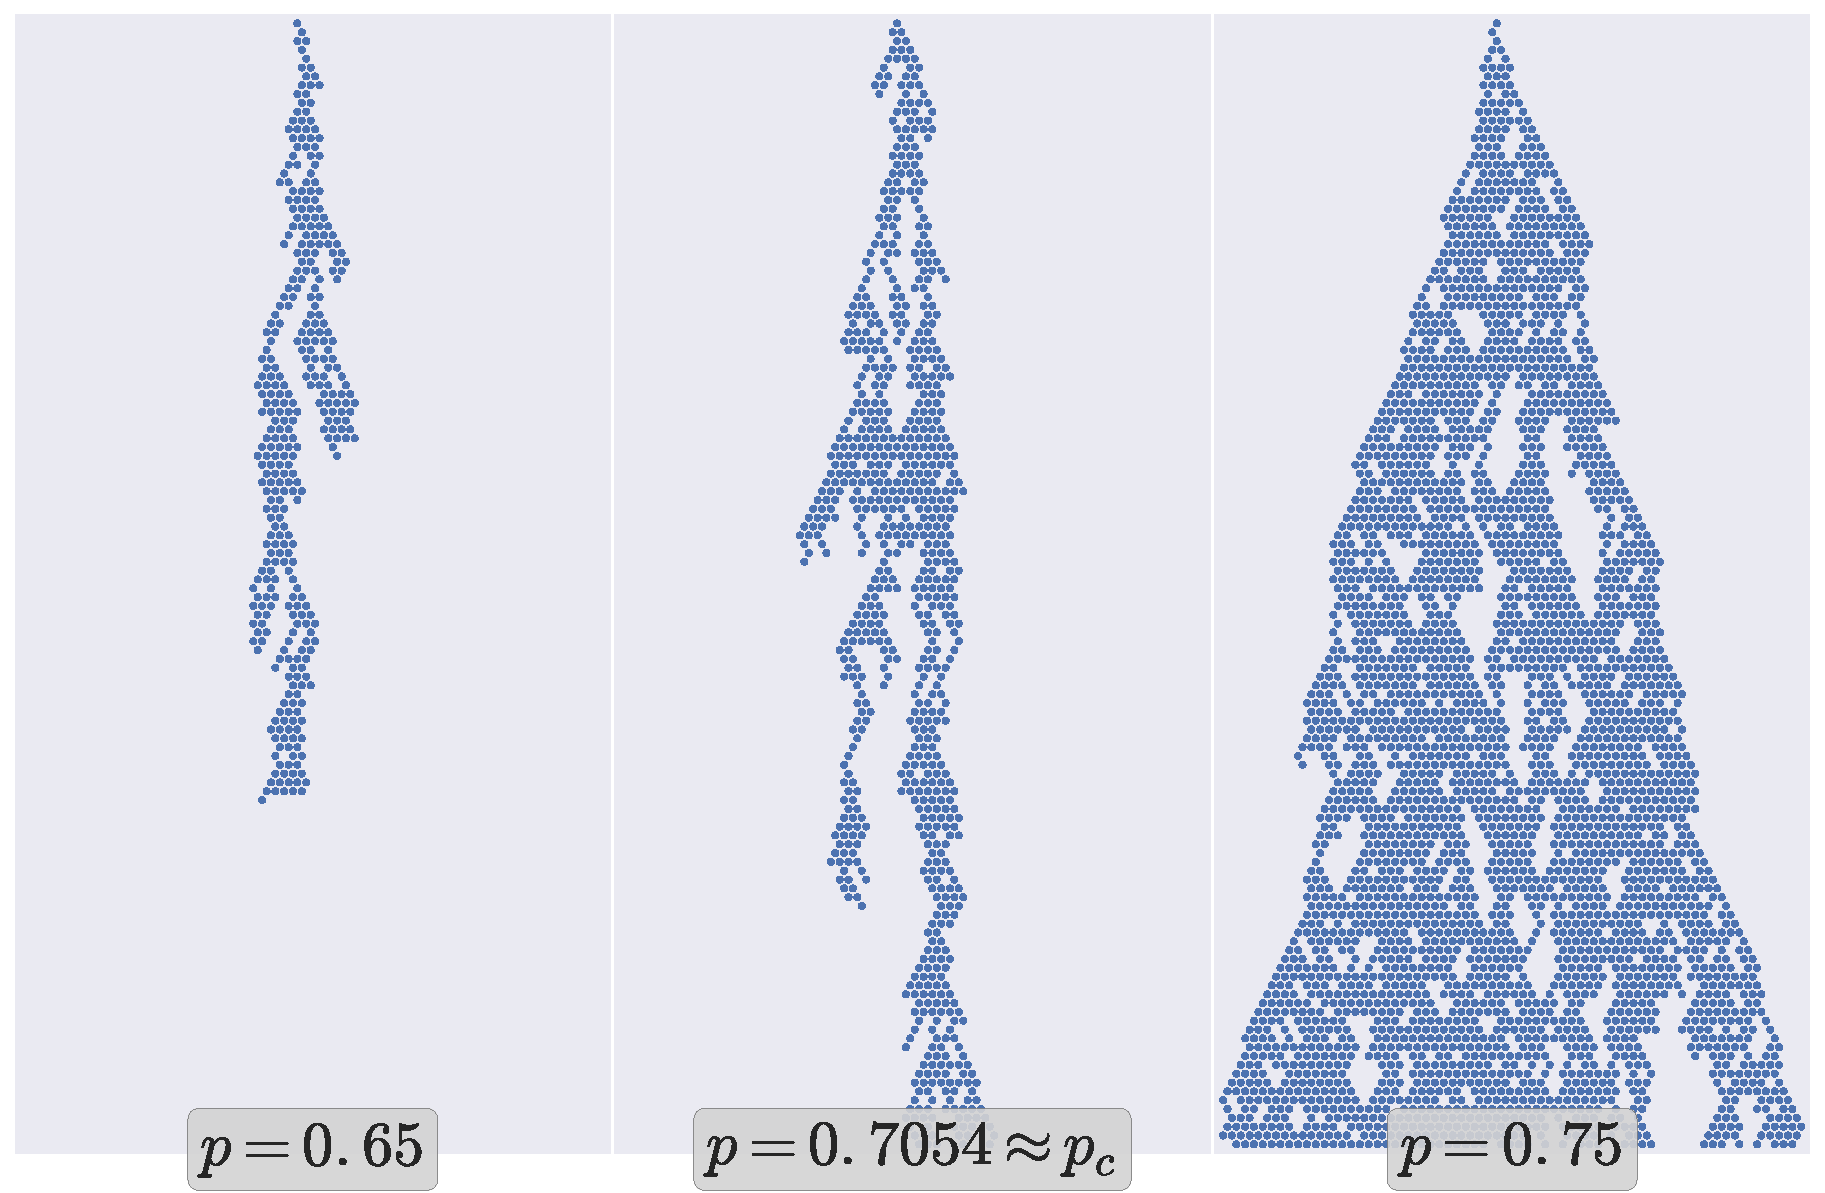
\includegraphics[scale=0.5]{chapters/ch5-anis/figs/dperco}
\end{center}
\caption{Three realizations of site directed percolation on a square lattice
    (here the time flows downwards). Being a absorbing phase transition model,
    the system have a probability of entering a state that it cannot leave, in
    this case a fully unoccupied state, like it happens in the left panel.
    Above the critical point however the probability of reaching an absorbing
    state becomes vanishing.}
\label{fig:dperco}
\end{figure}

\begin{figure}
\begin{center}
    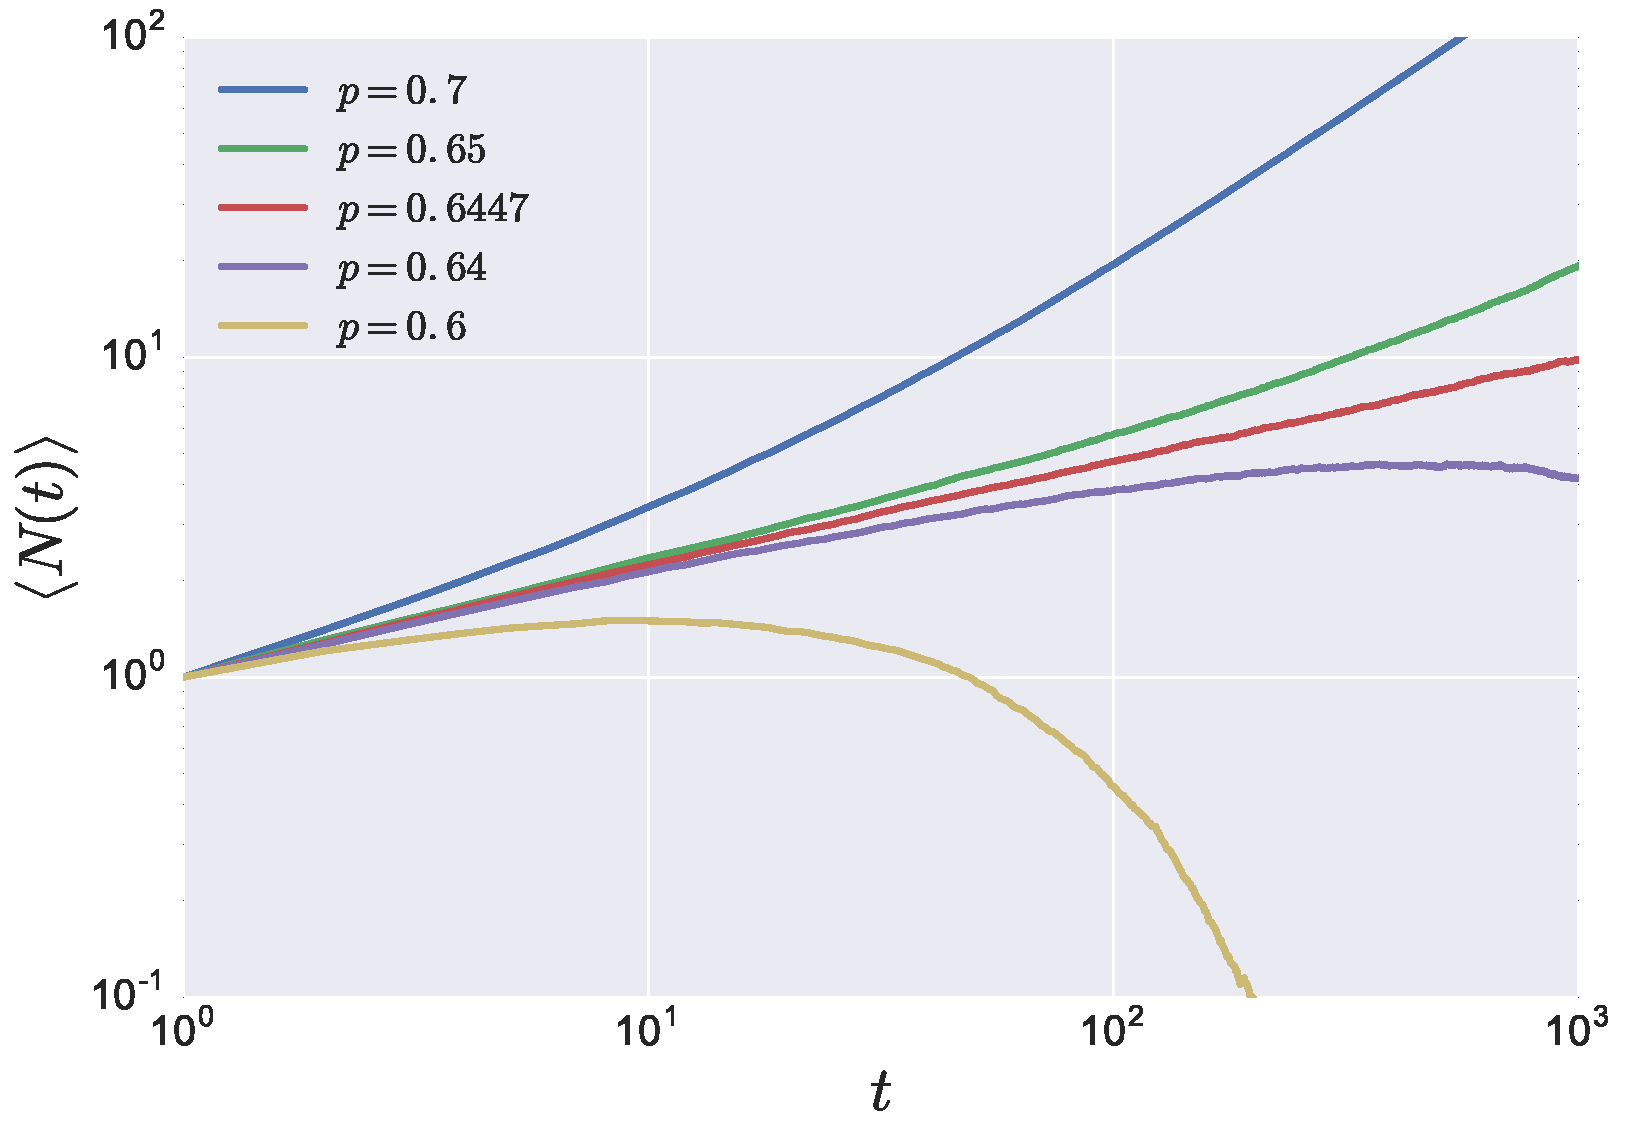
\includegraphics[scale=0.5]{chapters/ch5-anis/figs/dperco_nt}
\end{center}
\caption{Expected population of bond directed percolation as a function of time
    for various values of $p$. The critical point ($p_c\approx0.6447$) is the
    lowest value of $p$ such that $\lim_{t\rightarrow\infty}\left\langle
    N(t)\right\rangle>0$.}
\label{fig:dperco_nt}
\end{figure}


\section{Multi-Layered Percolation}
\label{sec:mlp}

Another universality class of strongly anisotropic phase transition is yet
another variation of the percolation model. Its aim is to model the structure
of stratified media, like layered porous rocks. Introduced by Dayan et al.\,
they suggested a percolation model for anisotropic multi-layered porous media
in which different layers may have different physical properties such as
density and porosity. Disordered systems such as layered fractured rocks are in
general anisotropic, i.e.\ physical properties such as density or porosity may
vary over the different layers.

In this model we take a $d$-dimensional lattice composed of several
$(d-1)$-dimensional sub-lattices (or layers) arranged in sequence, as if
they're stacked one over the other. Following convention, we'll call the axis
perpendicular to the layers the $y$-axis. We then perform the usual percolation
process by randomly occupying the lattice sites. The key difference here is
that each layer has its own occupation probability $p(y)$.
For simplicity, it is common to take a two-probability approach, where
each layer can have one of two values $p_1$ and $p_2$. These are
the control parameters of the model, where the line $p_1=p_2$ represent
the regular isotropic percolation. The larger the difference between
$p_1$ and $p_2$ the more accentuated if the anisotropy of the systems.
To this effect it is common to reparametrize the control parameter
by defining
\begin{equation}
    \bar{p}=\frac{p_1 + p_2}{2}\;\;\;\;\;\;\;\Delta=\frac{p_1 - p_2}{2}
\end{equation}
such that $p_1 = \bar{p} + \Delta$ and $p_2 = \bar{p} - \Delta$. 
The parameter $\Delta$ can take any value in the interval $[0.0,0.5]$,
and represents the degree of anisotropy of the system, which $\Delta=0$
is the isotropic case. 

As is expected, this model presents a second-order phase transition.
To determine the $\bar{p}_c(\Delta)$, Dayan et al.\ made use of the
cluster perimeter method.

We generate various cluster perimeters using the exploration method described
in Sec.~[???]. Making use of the fact that at the critical point a cluster
perimeter have equal chances of being an external or an internal border. We
generate several cluster perimeter and count the ration $R(\bar{p}, \Delta)$
between the number of realizations where the path was an internal perimeter and
the number of realizations where it was an external perimeter. The critical
point is such that $R(\bar{p}_c, \Delta_c)=1$. In the case of a square lattice
(the one studied by Dayan), we observe that there is a function
$\bar{p}_c(\Delta)$ that defines the border between the percolating and
non-percolating phases. This result can be seen in Fig.~[???]. Somewhat
surprisingly the same method was performed for the triangular lattice, and we
observed that $\bar{p}_c=0.5$ independent of the value of $\Delta$.

\begin{figure}
\begin{center}
    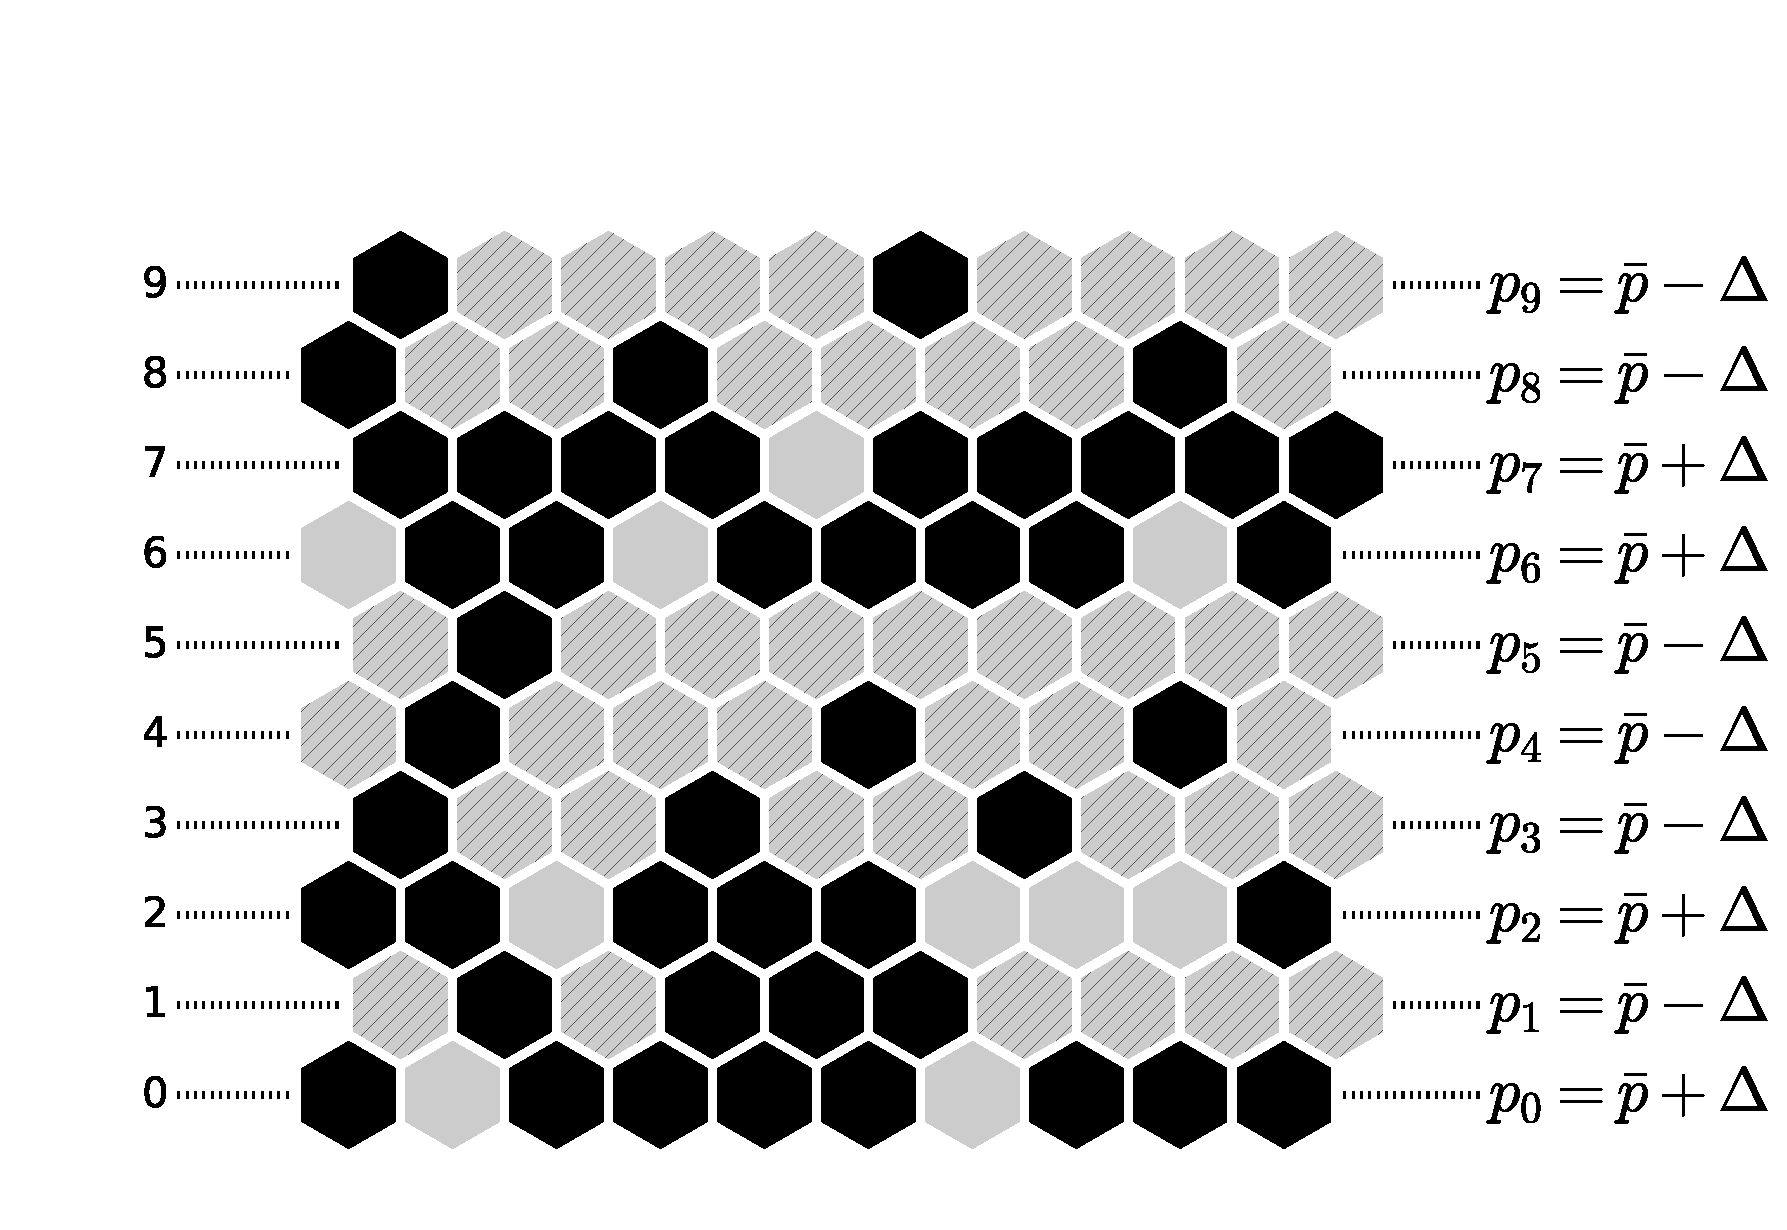
\includegraphics[scale=0.4]{chapters/ch5-anis/figs/mlperco_explain}
\end{center}
\caption{Schematic representation of the multi-layered percolation model. Each
    layer (numbered $0$ through $9$ here) gets one of two probabilities of
    occupation ($\bar{p}\pm\Delta$), chosen randomly with equal probabilities.
    Otherwise, the percolation process goes as usual, occupying each site
    according to the probabilities of each layer.}
\label{fig:mlperco_explain}
\end{figure}

\begin{figure}
\begin{center}
    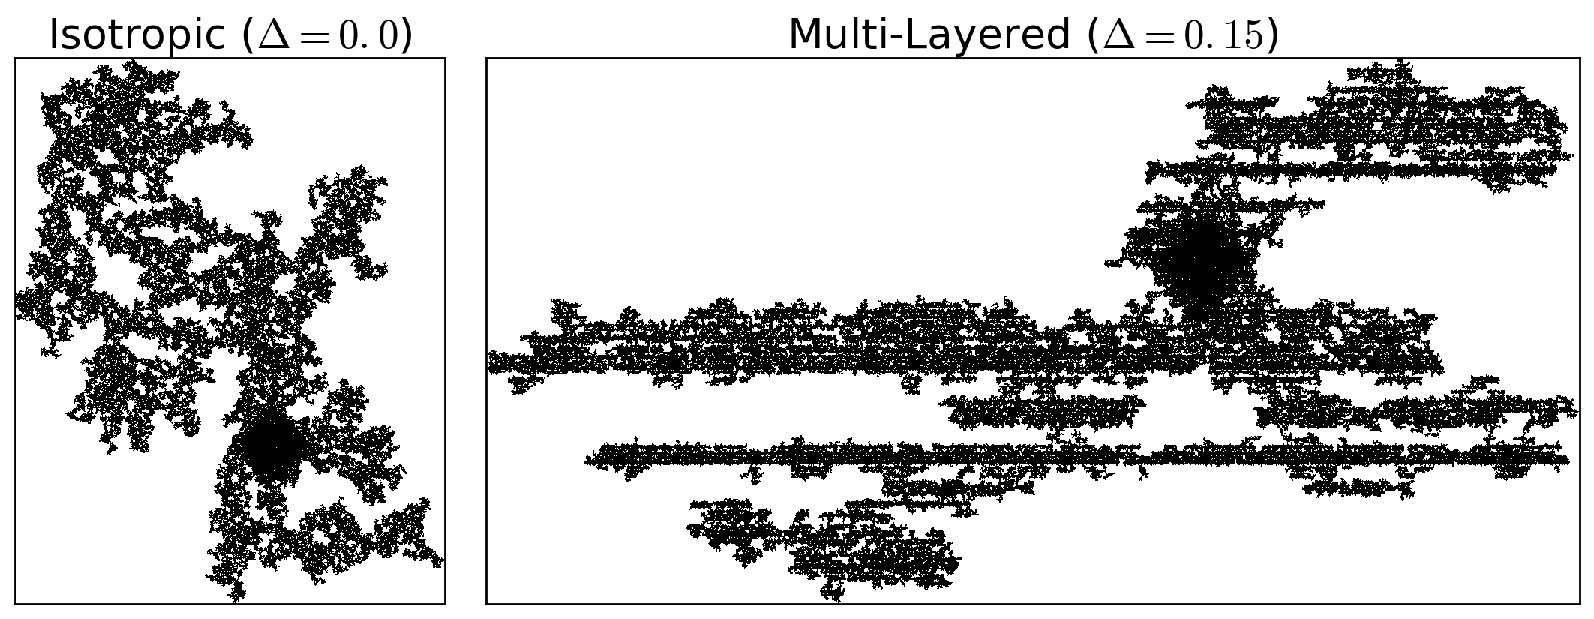
\includegraphics[scale=0.6]{chapters/ch5-anis/figs/mlp_cluster}
\end{center}
\caption{A comparison of clusters of occupied sites in both isotropic and
    multi-layered percolation at their critical points. They were generated
    using the self-organized percolation algorithm [???] (the dense ``core''
    found on both clusters is an artifact of this method). The stratified
    nature of the multi-layered percolation makes itself evident even for the
    relatively low value of $\Delta$ used here.}
\label{fig:mlp_cluster}
\end{figure}

\begin{figure}
\begin{center}
    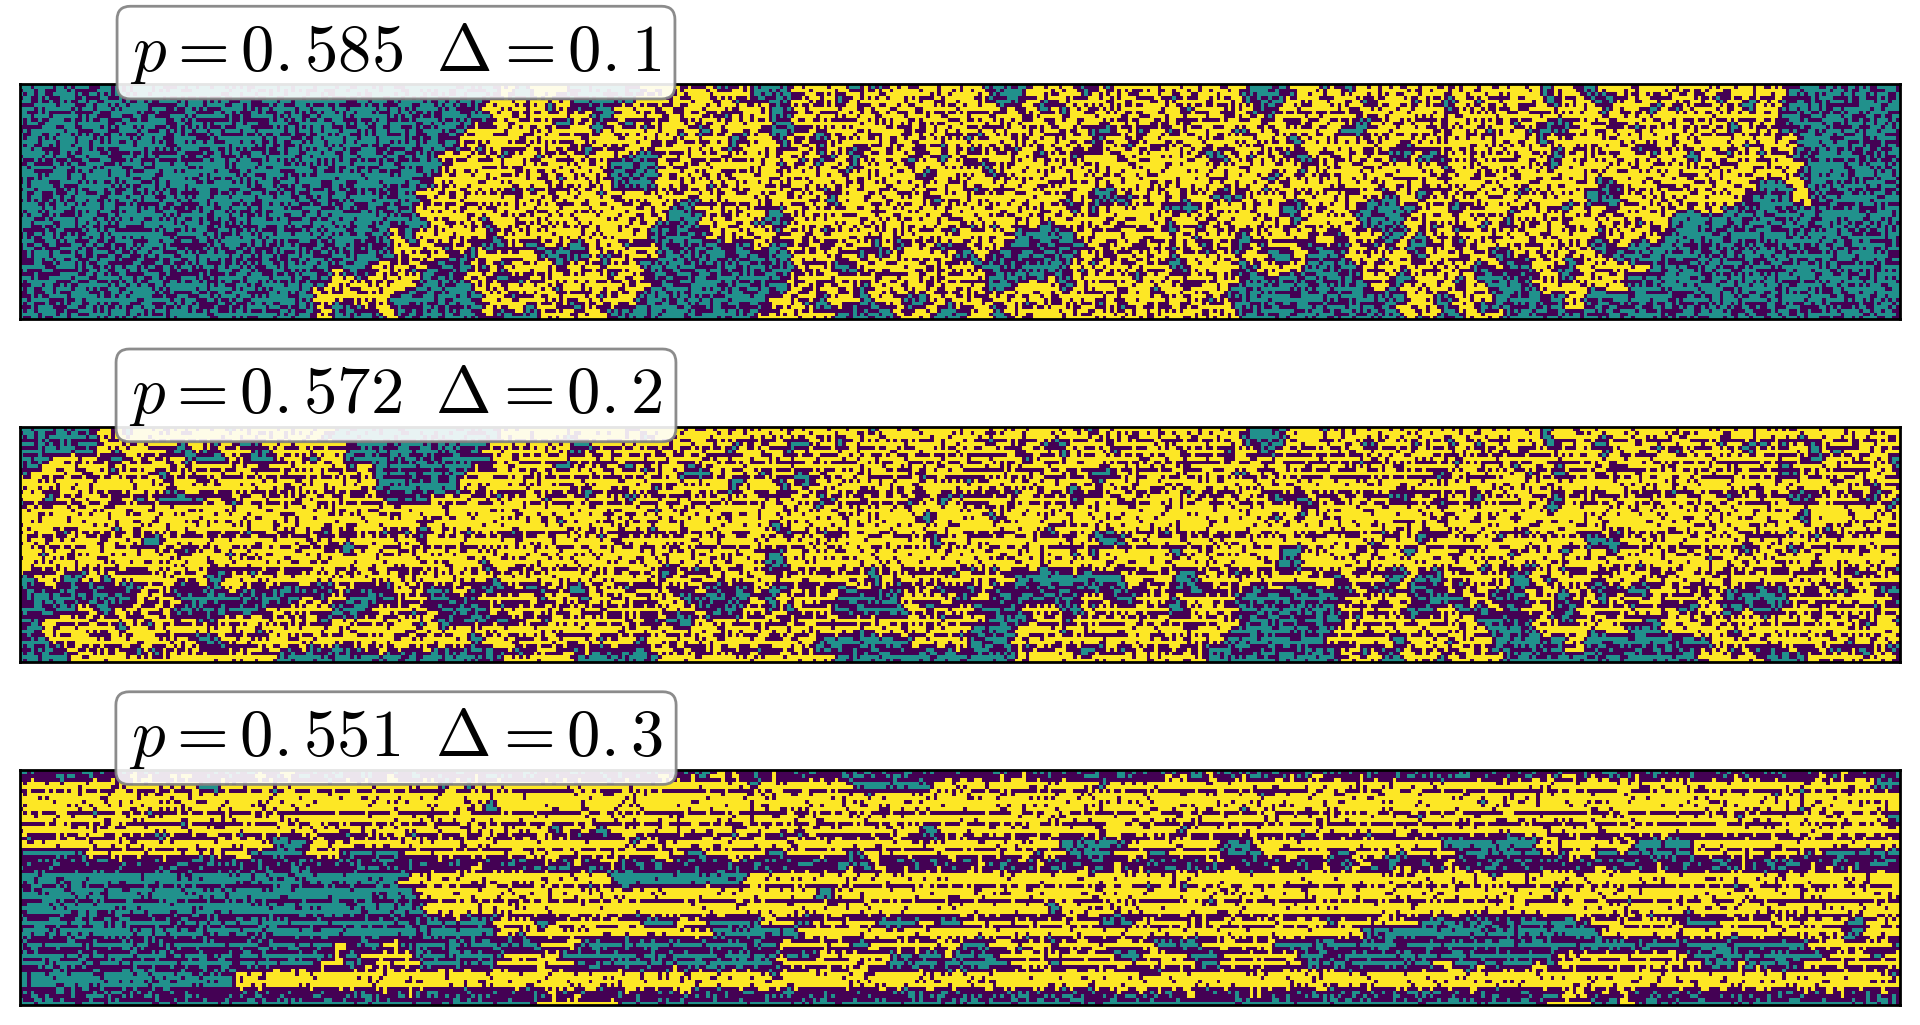
\includegraphics[scale=0.6]{chapters/ch5-anis/figs/mlperco}
\end{center}
\caption{Three realizations of the multi-layered percolation model in the
    square lattice. Black sites are unoccupied, dark cyan sites are occupied
    and yellow sites are represent the largest cluster of the system. All
    three realizations are in the critical point. The larger the value of
    $\Delta$, the more anisotropic is the system, and the multi-layered
    structure of the system becomes more evident.}
\label{fig:mlperco}
\end{figure}

\begin{figure}
\begin{center}
    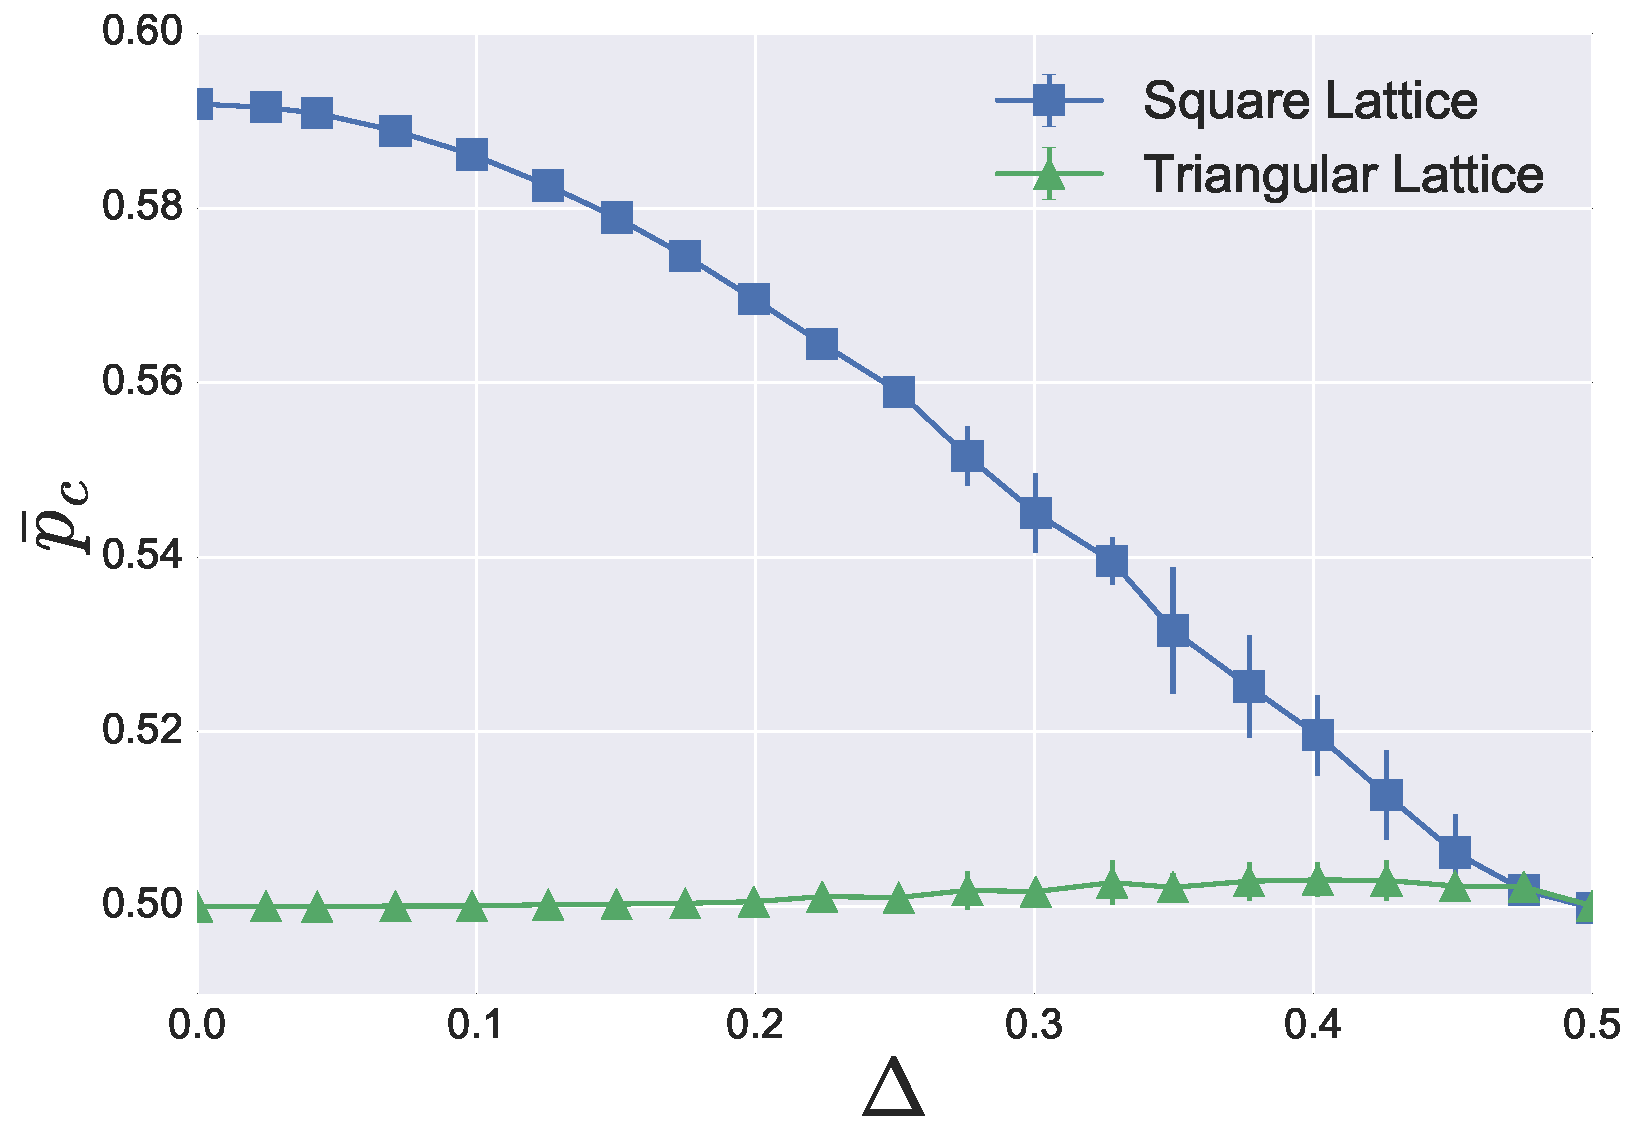
\includegraphics[scale=0.4]{chapters/ch5-anis/figs/mlp_ps}
\end{center}
\caption{Phase space of the multi-layered percolation model for both square and
    triangular lattices. They were computed using the cluster perimeter method.
    The square lattice result follow the results by Dayan et al.\ [???].
    Somewhat surprisingly we found that in the triangular lattice
    $\bar{p}_c=0.5$ for every value of $\Delta$.}
\label{fig:mlp_ps}
\end{figure}
